\documentclass[11pt]{article}
\usepackage{graphicx}
\usepackage{subcaption}
\usepackage{wrapfig}
\title{Ubiquitous Genomics: Hackathon2}

\author{
  Maya Anand\\ mva2112@columbia.edu \and
  Anne Bozack\\ akb2134@cumc.columbia.edu \and
  Cheyenne Parsley\\ cep2141@columbia.edu \and
  Robert Piccone\\ rap2186@columbia.edu \and
  Daniel Speyer\\ dls2192@columbia.edu}
\begin{document}
\maketitle
\section*{Problem 1}
Number of 2D reads classified as failed: 257\\
Number of 2D reads classified as passed: 1082\\
\section*{Problem 2}
\begin{wrapfigure}{r}{2.5in}
  \vspace{-20pt}
  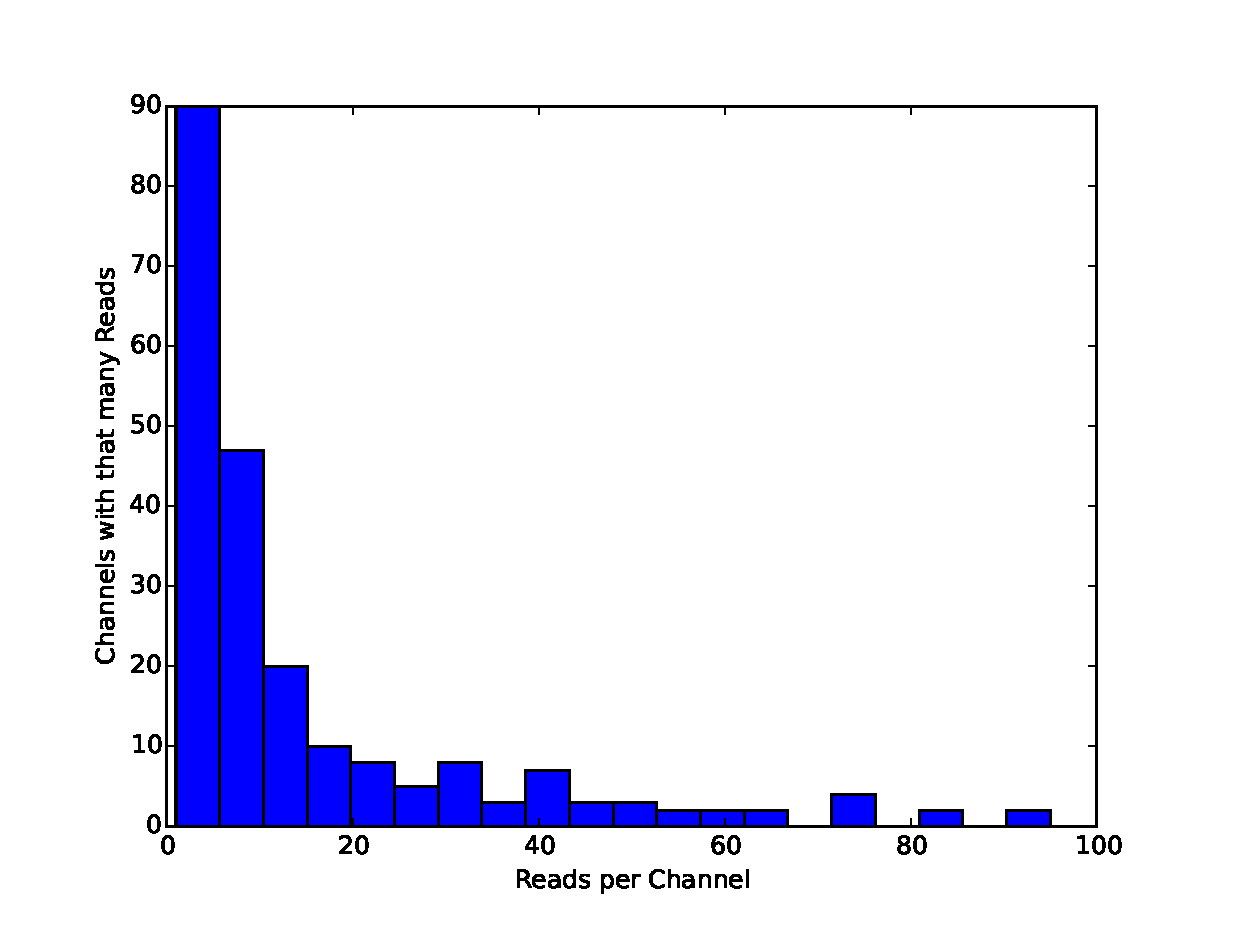
\includegraphics[width=2.5in]{part2hist}
  \vspace{-20pt}
\end{wrapfigure}
1 channels had at least one read, and 1 had at least five.  
This compares with 434 ``active'' channels during initialization, and 651 immediately after loading fuel

The average channel had 2520.0 reads. 
Channel 29 had 2520 reads, which was the most.
\section*{Problem 3}
\subsection*{Failed Reads}

        The following histograms show the length distribution of 2D and 1D reads for fails.

        
        \begin{tabular}{cc}
          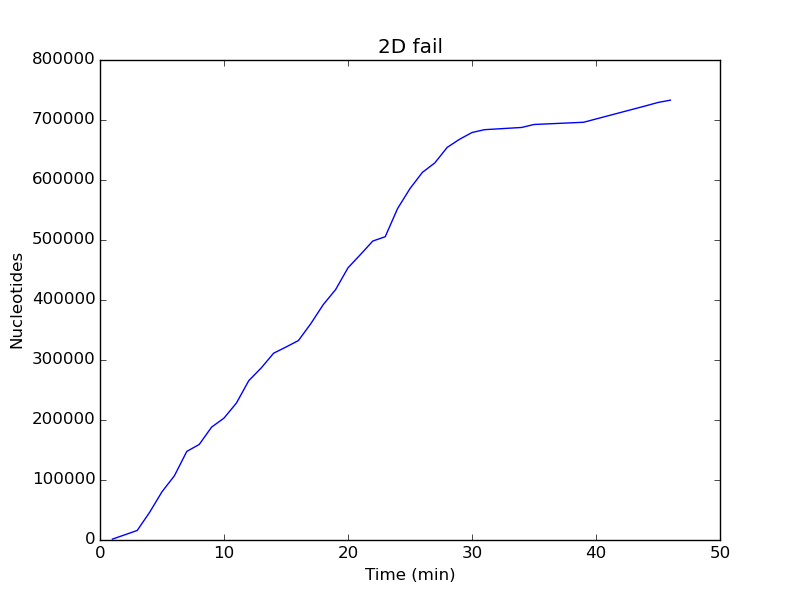
\includegraphics[width=.48\textwidth]{failcum2D}
          &
          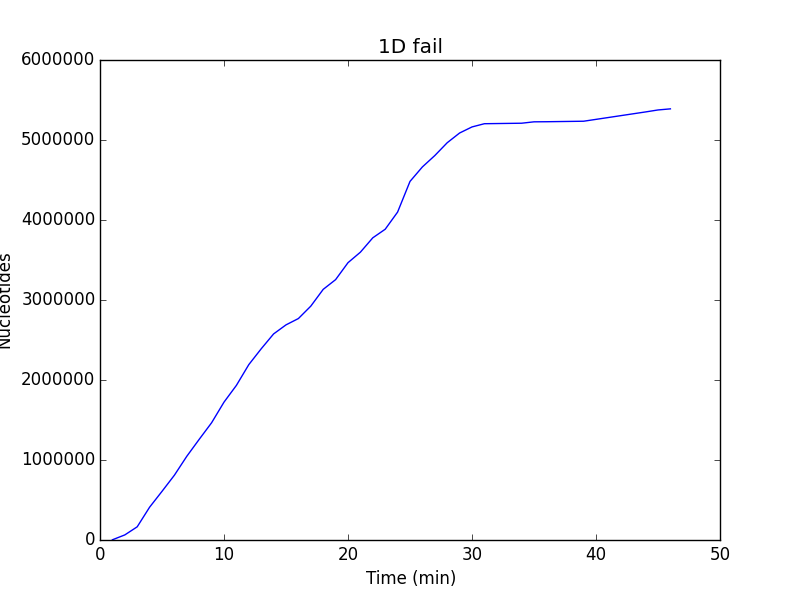
\includegraphics[width=.48\textwidth]{failcum1D}
          \\
          2D Reads
          &
          1D Reads
        \end{tabular}

\subsection*{Passed Reads}

        The following histograms show the length distribution of 2D and 1D reads for passes.

        
        \begin{tabular}{cc}
          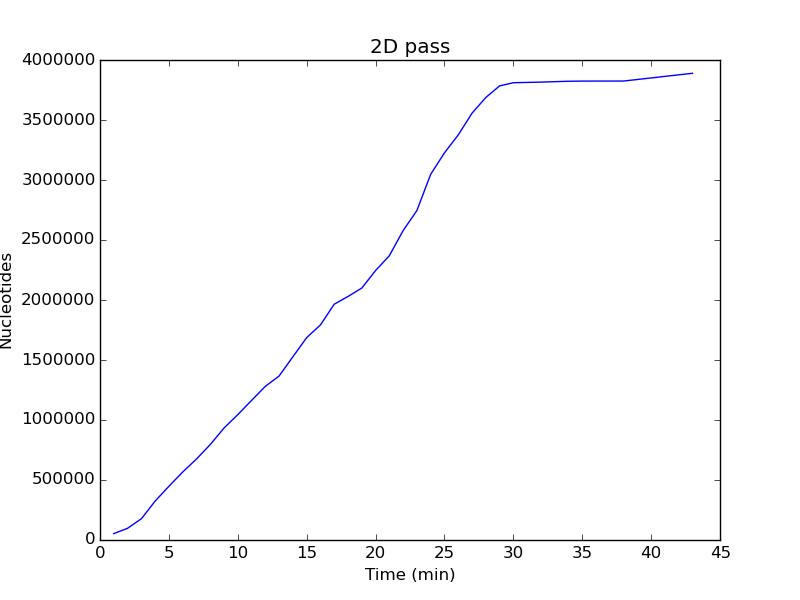
\includegraphics[width=.48\textwidth]{passcum2D}
          &
          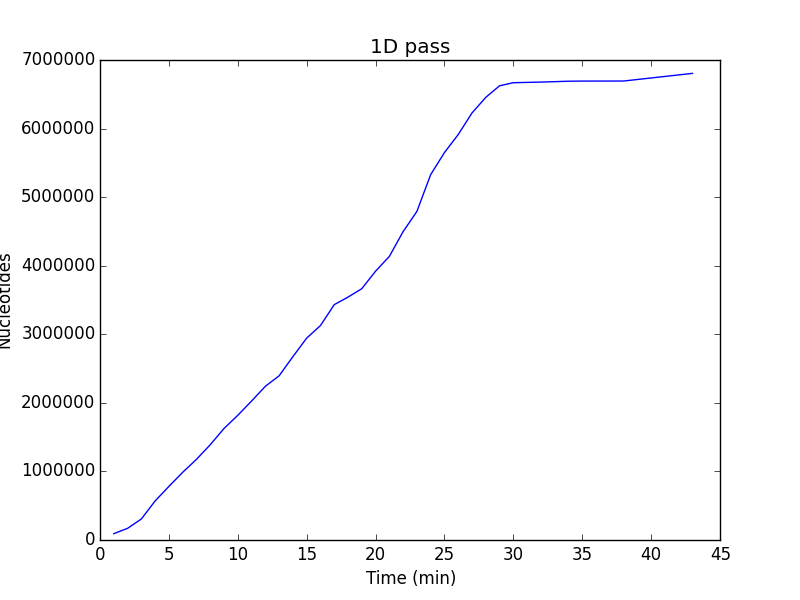
\includegraphics[width=.48\textwidth]{passcum1D}
          \\
          2D Reads
          &
          1D Reads
        \end{tabular}
\section*{Problem 4}
\subsection*{2D reads}

        The following histograms show the length distribution of 2D reads for passes and fails.

        
        \begin{tabular}{cc}
          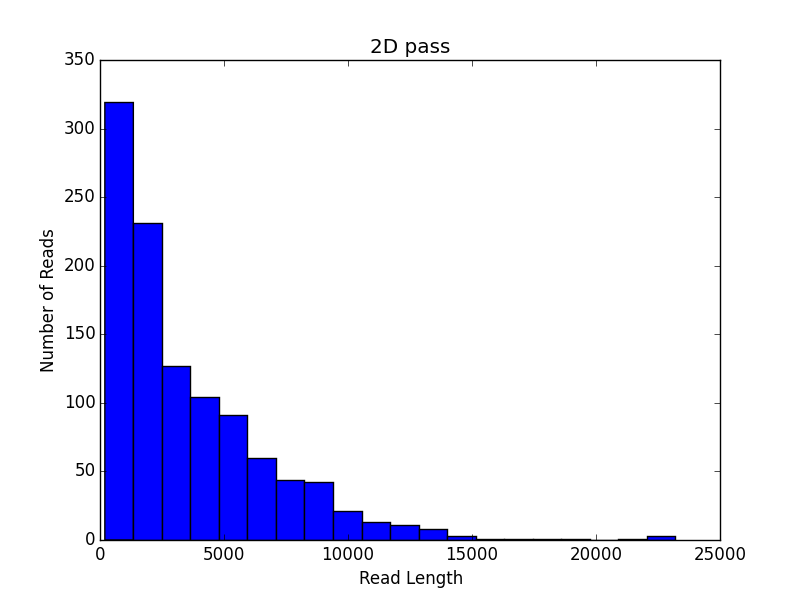
\includegraphics[width=.48\textwidth]{2Dpasses}
          &
          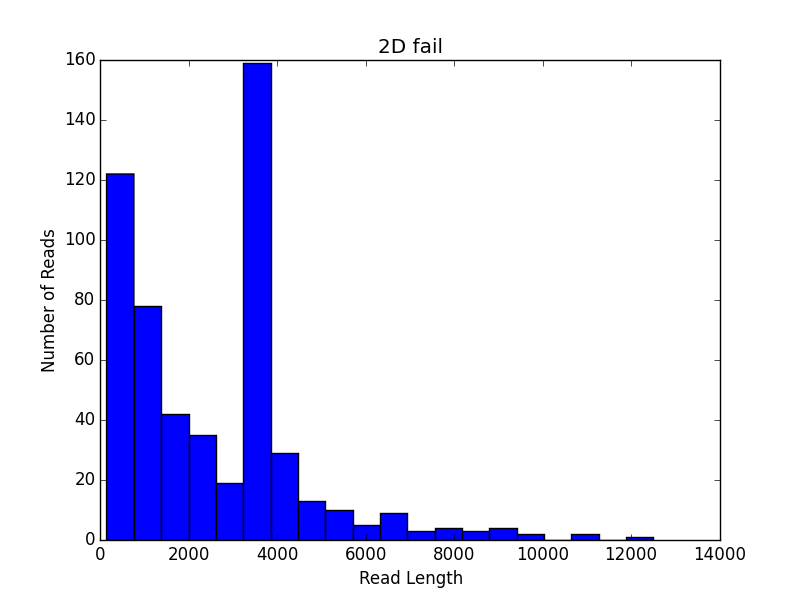
\includegraphics[width=.48\textwidth]{2Dfailures}
          \\
          Passed Reads
          &
          Failed Reads
        \end{tabular}
\section*{Problem 5}

LONGEST PASSED 2D READ\\
From file: MINION02\_Hackathon2\_group4\_TeamAWESOME\_4029\_1\_ch9\_file8\_strand.fast5\\
Number of nucleotides: 23196\\

LONGEST FAILED 2D READ\\
From file: MINION02\_Hackathon2\_group4\_TeamAWESOME\_4029\_1\_ch360\_file3\_strand.fast5\\
Number of nucleotides: 13419\\
\end{document}
